% ALU symbol preview
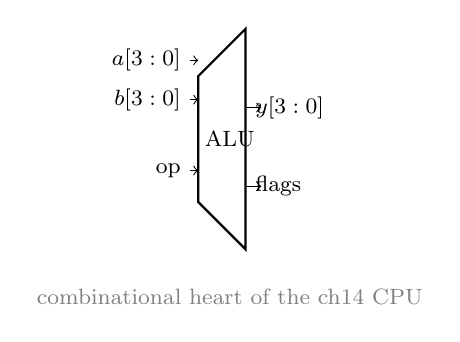
\begin{tikzpicture}[font=\footnotesize]
\draw[thick] (0,0) -- (0,1.6) -- (0.6,2.2) -- (0.6,-0.6) -- cycle;
\node at (0.4,0.8) {ALU};
\node[left] at (-0.1,1.8) {$a[3:0]$}; \draw[->] (-0.1,1.8) -- (0,1.8);
\node[left] at (-0.1,1.3) {$b[3:0]$}; \draw[->] (-0.1,1.3) -- (0,1.3);
\node[left] at (-0.1,0.4) {op}; \draw[->] (-0.1,0.4) -- (0,0.4);
\node[right] at (0.6,1.2) {$y[3:0]$}; \draw[->] (0.6,1.2) -- (0.8,1.2);
\node[right] at (0.6,0.2) {flags}; \draw[->] (0.6,0.2) -- (0.8,0.2);
\node[gray] at (0.4,-1.2) {combinational heart of the ch14 CPU};
\end{tikzpicture}
